\documentclass{article}
\usepackage{graphicx}
\usepackage[margin=1.5cm]{geometry}
\usepackage{amsmath}

\begin{document}

\title{Thursday Reading Assessment: Unit 0 part II, Electric Potential}
\author{Prof. Jordan C. Hanson}

\maketitle

\section{Memory Bank}

\begin{itemize}
\item $PE = q V$ ... Relationship between potential energy, charge, and voltage.
\item $V_{AB} = Ed$ ... Relationship between voltage between points A and B, a distance $d$ apart, for a constant E-field $E$.
\end{itemize}

\section{Voltage and Electric Field}

\begin{enumerate}
\item If the electric field is 2.5 kV/m in between the plates in Fig. \ref{fig:plates}, and the plates are separated by $d = 0.1$ m, what is the voltage between the plates? \\ \vspace{1cm}
\begin{figure}[ht]
\centering
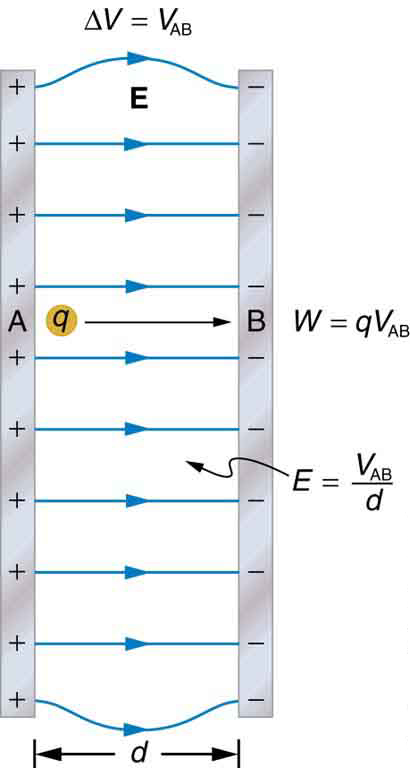
\includegraphics[width=0.15\textwidth]{plates.jpeg}
\caption{\label{fig:plates} The relationship between potential energy and voltage.}
\end{figure}
\item Consider Fig. \ref{fig:plates}, but instead let the voltage be 1 kV, and $d = 0.05$ m.  What is the magnitude of the electric field between the plates? \\ \vspace{1cm}
\item Consider Fig. \ref{fig:plates}, but instead let the E field be 0.6 kV/m, and the voltage be 400 V.  What is the distance between the plates? \\ \vspace{1cm}
\item (Same numbers as the prior example).  What if a particle of charge $q = +1$ nC and mass $10^{-9}$ kg was released on the left side of the system.  (a) What would be the potential energy?  (b) What is the final kinetic energy?
\end{enumerate}

\end{document}
